%% android.tex
%% by Simon Danner

% The Computer Society requires 12pt.
\documentclass[12pt,journal,compsoc]{IEEEtran}
\usepackage[ngerman]{babel}   
\usepackage[utf8]{inputenc}   % UTF8-Kodierung für Umlaute
\usepackage{hyperref}         % Hyperlinks
\usepackage{listings}
\usepackage{graphicx}

\clubpenalty = 10000           % Keine "Schusterjungen"
\widowpenalty = 10000          % Keine "Hurenkinder"

\selectlanguage{ngerman}

\newcommand{\Monat}{%
\ifcase\month
 Monat 0 \or Januar \or Februar \or März  \or April\or Mai\or Juni\or Juli\or August\or 
 September\or Oktober\or November\or Dezember
\fi}


\newcommand{\paperTitle}{
	Connecting Android powered devices to the external world	
}

\newcommand{\paperSubTitle}{
}

\newcommand{\absatz}{
	\parskip 12pt
}

\newcommand{\paperAuthor}{Simon~Danner}

\newcommand{\todo}[1]{
    \textbf{Todo:}#1
}


% korrigiere Silbentrennung % Kann man auch dazu verwendet die Silbentrennung zu deaktivieren
\hyphenation{op-tical net-works semi-conduc-tor}
% Silbentrennung für ein einzelnes Wort deaktivieren geht mit:
% \mbox{wort}


% Bei einem zwei Spalten Layout versucht Latex auf beide Seiten die gleiche Texthöhe hinzubekommen
% Dies verursacht leider manchmal Leeräume z. B. zwischen der Überschrift und dem Text
% Mit der Option \raggedbottom kann dies unterbunden werdne
% Hat aber den Nachteil das das Dokument so einen unregelmäßigen Seitenfuß hat
% Aber immer noch besser wie die Leerräume
%\raggedbottom

\begin{document}

\title{\paperTitle \\ \paperSubTitle }
\author{\paperAuthor,~\IEEEmembership{ AI7 }}% <-this % stops a space

% The paper headers
% \markboth{Journal of \LaTeX\ Class Files,~Vol.~6, No.~1, January~2007}
% {Shell \MakeLowercase{\textit{et al.}}: Bare Advanced Demo of IEEEtran.cls for Journals}

\IEEEtitleabstractindextext{%
	\begin{abstract}
		TODO Abstract

	\end{abstract}

	% Note that keywords are not normally used for peerreview papers.
	\begin{IEEEkeywords}
		Android, Hardware, Arduino, IOIO ADK, ADK 2012, AOA, Bluetooth LE  
	\end{IEEEkeywords}
}

\maketitle

\section{Einleitung}


\IEEEPARstart{A}{}ndroid ist mit einem Marktanteil von ca. 85\% nach IDC das zur Zeit am weitesten verbreitete Smartphone und Tablet Betriebssystem.\cite{marketshare}
Android wird auf Smartphones, Tablets, Smartwatches, Fernsehern und anderen Geräten verwendet.
Da die Nutzer solcher Geräte, diese oft rund um die Uhr bei sich tragen, bietet es sich an, diese Geräte zur Steuerung von anderen elektronischen Geräten zu nutzen.





% Datum
\hfill{\the\day~\Monat, \the\year  }

\section{Allgemeines}
TODO Nutzen, Entwicklung

\section{Anbindungsmöglichkeiten}
Mittlerweile gibt es mehrere Möglichkeiten, Hardware mit Android Geräten zu verbinden. 
Diese decken ein großes Spektrum an Anwendungsmöglichkeiten ab, wobei jede Vorteile und Nachteile bei bestimmten Anwendungen besitzt.
Nach ersten experimentellen Ansätzen von Hobbyentwicklern und einzelnen Firmen, hat auch Google den Nutzen einfacher Verbindung mit externen Geräten 
erkannt und bietet seit 2011 offiziell unterstützte Möglichkeiten, dies zu realisieren. 

\section{ADB (Android Debug Bridge)}
\subsection{Grundlagen}
Die Android Debug Bridge ist eine Softwaresuite mit der es möglich ist, von Host PCs mit Android Geräten zu kommunizieren.
Der Hauptnutzen besteht darin, Android Applikationen in einem virtuellen Gerät (Emulator) oder direkt auf echten Geräten zu debuggen.
Dabei wird auf dem Host ein Server gestartet, welcher die Kommunikation zwischen Host und Endgerät übernimmt. 

Die Clients (z.B. das adb command line tool, oder IDEs wie Android Studio), verbinden sich mit dem Server und senden Befehle an das über USB (oder Wifi) mit dem Server verbundene Endgerät.
Auf den Endgeräten oder im Emulator läuft im Hintergrund ein Dienst, der die Kommandos vom Server entgegennimmt und antwortet. Die Kommunikation mit dem Server läuft über TCP,
was es Clients ermöglicht sich über das Netzwerk mit Servern zu verbinden. (Siehe Abbildung \ref{adb})
\begin{figure}
	\centering
	\caption{Android Debug Bridge Architektur}
	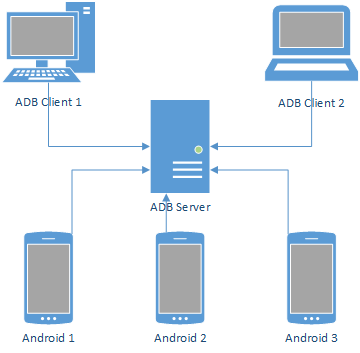
\includegraphics[width=0.4\textwidth]{media/adb.png}	
	\label{adb}
\end{figure}

Der ADB Dienst auf den Endgeräten muss explizit durch den Nutzer aktiviert werden, bevor er benutzt werden kann.
Da adb für das debuggen von Apps, also für Softwareentwickler konzipiert ist, stellt dies im allgemeinen kein Usability Problem dar. 
Das ADB Protokoll selbst ist sehr einfach gehalten, so dass eine eigenständige Reimplementierung möglich ist.
Die Kommunikation läuft dabei über einfache Message Pakete, in denen verschiedene Kommandos enthalten sein können.
\lstset{language=C,
	basicstyle=\ttfamily\scriptsize
}
\lstinputlisting{code/adb_struct_message.c}
  

\subsection{Verwendung mit externen Geräten}
Außer dem benutzten der ADB zum debuggen, kann die Architektur auch benutzt werden, um eigene Kommunikationsprotokolle zu implementieren.
Dabei wird das eigene Protokoll als eine Zusatzschicht über adb, in Form von Kommandos implementiert. TODO ??


TODO wann von wem zur Device kommunikation ?? --> IOIO

\section{Bluetooth}
Mit dem Bluetooth Standard ist es seit den 90er Jahren möglich, Geräte miteinander über Funktechnik zu verbinden. Bluetoothschnittstellen gehören schon lange zur Standardaustattung bei Handys und Smartphones.
Zur Anbindung von eigen entwickelter Elektronik ist Bluetooth aber nur bedingt geeignet, da die elektronische Umsetzung recht teuere und komplexe Chips erfordert. Außerdem ist der Stromverbrauch auf Android Seite recht hoch.
\subsection{Bluetooth Low Energy}
Bluetooth Low Energy, kurz BLE ist seit 2009 optionaler Teil des Bluetooth Standard Version 4.0. 
Ziel von BLE ist es, den Stromverbrauch mittels darauf optimierter Protokolle und anderer Einschränkungen gegenüber Bluetooth zu verringern.
In Smartphones wurde BLE in nennenswertem Umfang zuerst von Apple mit iOS 5 ( Oktober 2011)unterstützt.
Von Android wird Bluetooth LE ab der Version 4.3 (Release Juli 2013) unterstützt.
BLE ermöglicht es Chips zu entwickeln, die nur dieses Protokoll unterstützen (kein volles Bluetooth TODO), was die Chips für Hardwarehersteller billiger und einfacher zu verwenden macht.
Bluetooth LE Geräte stellen dabei standardisierte Services und Profile bereit, die verschiedene Anwendungsbereiche abdecken.
So gibt es zum Beispiel Services  
\cite{bluetooth}

\section{NFC TODO}

\section{USB OTG}

\section{Audio}
Android unterstützt Entwickler bei der Einbindung von Audio Geräten. Das Verwalten der Hardware wird von Android komplett übernommen.
Falls gewünscht, können Entwickler von Audio Applikationen über den AudioManager herausfinden, was für Geräte angeschlossen sind. So kann man zum Beispiel die Lautstärke anpassen wenn ein Bluetooth Headset verbunden wird, oder Kopfhörer entfernt werden.

Da die Verwendung von Audio Geräten fast automatisch abläuft, wird hier nicht weiter auf Audio Geräte eingegangen.

Historisch gab es einige Entwicklungen die Audioausgabe zur Übermittlung an externe Geräte zu verwenden. Diese sind jedoch in Anbetracht heutiger Möglichkeiten eher als historische Kuriositäten von Bastlern zu sehen.
Ein Beispiel für ein solches Projekt ist Project HiJack \cite{hijack} , welches eine Hard- und Software Plattform zur Übermittlung von Signalen und Verarbeitung dieser auf Microcontrolern unter iOS sowie Android entwickelte.
Die Probleme hierbei sind vor allem die analoge Übertragung und die relativ begrenzte Bandbreite.


\section{AOA (Android OpenAccessory)}
Android OpenAccessory ist der Name eines von Google entwickelten Protokolls, was 
dezidiert für die Anbindung von externen Geräten an Android Geräte entwickelt wurde.
Die erste Version (ADK 2011) wurde im Mai 2011 vorgestellt.

Das ADK besteht aus einer Hardware Referenz Plattform, sowie Source Code für diese, damit 
Entwickler einfach Hardware und Software anpassen und erweitern können.
\cite{developaoa}
\subsection{Ziel}
Ziel Googles ist es mithilfe des AOA einen einheitlichen Standard zur Verbindung von externen Geräten mit Android Geräten zu etablieren.
Dies führt dazu, dass Endanwender ohne auf spezielle Gerät Kombinationen verwendet zu müssen, externe Hardware kaufen und benutzen können.
Google veröffentlichte bisher (Stand September 2014) zwei Versionen des ADKs, 2011 und 2012. 

\subsection{Vergleich mit ADB}
Gegenüber der Kommunikation über das ADB Protokoll, bietet AOA einige Vorteile. In \ref{table:vergl} sind einige Kenngrößen gegenüber gestellt. Der größte Vorteil der Benutzung von AOA gegenüber ADB, besteht darin, dass AOA nicht explizit vom Benutzer eingeschaltet werden muss und offiziell unterstützt wird.


\begin{table}
	\centering
	\caption{Vergleich ADB / AOA Quelle: \cite{comp}}
	\label{table:vergl}
	\begin{tabular}{c | c | c}
		& ADB & AOA \\ \hline
		Latenz & 4ms & 1ms \\ \hline
		Durchsatz & 300 KB/s & 600 KB/s \\ \hline
		Verfügbarkeit & alle Versionen & \textgreater 2.3.4 \\ \hline
	\end{tabular}
\end{table}


\subsection{ADK 2011}
Beim ADK 2011 wurde von Google eine
Referenz Plattform auf Basis eines Arduino Mega2560 Microcontroller System, welches ein USB Host Modul enthält, sowie eine Arduino Bibliothek zur Kommunikation über AOA mit fähigen Android Geräten veröffentlicht.
Durch die Benutzung des Arduino Controllers ermöglicht es Google, Hobby Entwicklern einen enfachen Einstieg in die Entwicklung von Accesoires, da diese Microcontroller sehr verbreitet und es viele Tools für diese Systeme gibt.
So ist die Programmierung mit der Arduino IDE möglich, welche durch einen C-Dialekt geschiet, welcher auch für Anfänger einfach verständlich ist.
Die Android seitige Funktionalität von AOA wurde in Android 2.3.4 (Release April 2011) und spätere Versionen integriert. 
Um mit dem ADK eigene Accesoires entwickeln zu können, muss das Board zunächst mit der von Google bereitgestellten Firmware, welche AOA implementiert geflasht werden.
Danach kann mit der Arduino IDE 
TODO Beispiele
\subsection{ADK 2012}
\subsubsection{Änderungen}
Im der 2012er Version des ADK ist die Hardware Platform gewechselt geworden. Nun dient ein Arduino kompatibles Board mit einem ARM Cortex M3, Sensoren für Licht, Farbe, Temperatur, Feuchtigkeit, Druck und Beschleunigung, einem Micro SD Card Slot und Bluetooth als Referenz.
Die neuen Sensoren und Verbindungsmöglichkeiten machen dieses Board noch attraktiver für Entwickler, welche eigene Hardwareerweiterungen vermeiden wollen.

Im ADK 2012 wurde die Möglichkeit von Audio Übertragungen über das AOA Protokoll hinzugefügt, wodurch Anwendungen in diesem Gebiet vereinfacht werden.
Außerdem kann AOA über Bluetooth verwendet werden. Hierfür wird das Bluetooth Serial Port Profile (SPP) zur Kommunikation genutzt. Für eigene Implementierungen muss somit ein Bluetoothchip der dieses Profil unterstützt verwendet werden.

\lstinputlisting[language=Java]{code/bluetooth.java}
In der Android App kann über die Android Bluetooth Schnittstelle eine Verbindung aufgebaut werden.
\lstinputlisting[language=Java]{code/bluetooth2.java}
Dann kann über Streams mit dem Gerät kommuniziert werden.

\subsection{Das AOA Protokoll}
Um mit einem Accesoire Gerät mit einem Android Gerät kommunizieren zu können, muss zunächst das Android Gerät in den richtigen Modus versetzt werden.
Dies geschiet durch einen Request 51 TODO, der zurückliefert welche Version des AOA Protokolls unterstützt wird. Falls keine Antwort zurückkommt, wird das verbundene Geräte ignoriert.
Wenn die Verbindung aufgebaut wurde, müssen geeignete USB Endpunkte gefunden werden. Endpunkte sind vom USB Interface bereitgestellte Transportmethoden. An sie können Daten übertragen werden.
Endpunkte werden von allen USB Geräten verwendet, die verschiedenen Typen sind im USB Standard beschrieben.
AOA benutzt Bulk-Endpunkte. Diese werden bei USB allgemein zum Transport von längeren Blockartigen Datenblöcken benutzt.

Bulk Transfers verwenden CRC zur Fehlererkennung und Korrektur. Es ist garantiert das übertragene Daten korrekt ankommen, es gibt allerdings keine Bandbreite oder Latenz Vorschriften.
\cite{usbbulk}
Nach dem die korrekten Endpunkte gefunden wurde, können sie von dem Accesoir zum senden von Daten verwendet werden.

Auf dem Androidgerät wird daraufhin eine Liste von Applikationen welche die AOA Api unterstüzten dem Benutzer gezeigt, dieser kann damit die zum aktuellen Accesoir passende Applikation starten, welche dann Daten austauschen kann. TODO echt?


Erkannt werden kann der Accesory Modus ist, wenn das USB-Interface eine Vendor ID 0x18D1 und eine Produkt ID von 0x2D00 oder 0x2D01 hat. 

\section{Beispiels AOA Anwendung}
Da Android OpenAccessory die von Google offiziell unterstütze API für die Anbindung externer Geräte ist, wird der Aufbau von einer solchen Applikation detallierter eingegangen.
\subsection{AOA Hardware}
Um mit AOA eine Anwendung mit Hardwarekomponente entwickeln zu können, braucht man ein kompatibles Hardwareboard.
Zurzeit können hierfür die von Google als Referenz Plattform bereitgestellten Arduinos, sowie einzelne andere Boards von Drittherstellern, wie z. B. das IOIO Board \cite{ioio}, das AOAA Kit von Embedded Artists\cite{aoaa},  TODO more examples , oder man entwickelt die Elektronik basierend auf der Dokumentation des Protokolls selbst\cite{aoaprotocol2}.
Für die Beispielsanwendung wird das IOIO Board benutzt.

\subsection{IOIO Hardware}
Die erste Version des IOIO Boards wurde im September 2011 vorgestellt. Das Board wurde von Ytai Ben-Tsvi, einem Google Angestellten, für eigene Projekte im Rahmen der Google 20\% Zeit entwickelt und als Kooperation mit dem Elektronikunternehmen SparkFun produziert und verkauft.
Es war der erste Board, welches ohne Modifikationen an Android Geräten von diesen verwendet werden konnte, um damit externe Peripherie zu steuern.
Dies wurde über die Verwendung der Android Debug Bridge erreicht, welche als Übertragungsprotokoll verwendet wird.
Als weitere Protokollschicht wurde ein eigenes IOIO Protokoll entwickelt, mit dem einfache Kommandos übermittelt werden können.
So gibt es Kommanos wie \glqq Schalte Pin 1 ein\grqq, oder \glqq Lese Pin 3 analog\grqq, die durch entsprechende Methoden direkt in der zugehörigen IOIO Android Bibliothek aufgerufen werden können.

Als Microcontroller kommt ein PIC24F zum Einsatz, welcher auf Grund seiner vielen Anschlüsse und geringer Kosten gewählt wurde.
Das Board besitzt 48 Pins, welche als Digitale Inputs und Outputs angesteuert werden können. 16 dieser Pins können auch als analoge Inputs verwendet werden.
Zusätzlich können 9 PWM (Pulsweitenmodulation) Ausgänge verwendet werden.
Für die Kommunikation mit anderen Elektronischen Geräten stehen 4 UART Kanäle, 3 SPI Kanäle und 3 TWI Känale, welche mit I\textsuperscript{2}C kompatibel sind zur Verfügung.
Der Strom wird über ein externes 5V Volt Netzteil bereitgestellt, welches bis zu 1.5 Ampere liefern muss.

Die externe Stromversorgung ist praktisch, da sowohl das Androidgerät geladen werden kann, als auch Motoren oder ähnliches durch das Netzteil mitversorgt werden können.
Ziel der Neuentwicklung war vor allem, eine kostengünstige Möglichkeit, die gleichzeitig mit Standard Android Geräten verwendet werden kann, der Öffentlichkeit bereitzustellen.
Mit einem Preis von 50\textdollar{} ist das Projekt für Hardwarebastlereien und Prototypen geeignet.
Das Board besitzt einen USB Anschluss, welcher im Host Modus betrieben werden kann, was Voraussetzung für den Betrieb von ADB und AOA ist.

\subsubsection{IOIO-OTG}
Im Sommer 2012 wurde die zweite Version des IOIO Boards veröffentlicht.
Die größte Änderung ist die Möglichkeit das IOIO Board als USB OTG Device zu betreiben.
Dadurch kann das Board sowohl als USB Master (auch Host) als auch als USB Slave (auch Peripheral) verwendet werden.
Dies ermöglicht die Verbindung mit PCs, mit denen das Gerät auch direkt programmiert werden kann.
Dies vereinfacht den Entwicklungsprozess, da keine Android Applikation mehr auf dem Gerät installiert werden muss um Programme zu testen.
In der Java Bibliothek wurde diese Neuerung auch aufgenommen, so dass diese nicht nur unter Android laufen kann, sondern auch in der Standard JVM.
Außerdem konnten die Produktionskosten weiter gesenkt werden, die neue Version ist nun bei Partnerunternehmen für ca. 30\textdollar{} erhältlich.

\subsection{Vorhaben}

\subsection{Umsetzung}

\subsection{Erkenntnisse}





\section{Ausblick}
Zukunft TODO
\subsection{AOA}

\subsection{Bluetooth}

\subsection{NFC}
\section{Fazit}






\bibliographystyle{IEEEtran}
\bibliography{android_quotes}

% for the book
\nocite{*}
\end{document}

